\chapter{3D Modelling}
Sowohl die Charaktere als auch Assets wurden ausschlie"sslich in Blender gemodelt. Hierbei wurde sich stark an reellen Vorgaben, was Kleidung oder einpr"agsame Details betrifft, orientiert. Um den angestrebten Lowpoly-Stil konstant umzusetzen wurden teilweise erst Highpoly-Modelle erstellt um diese in der sogenannten ``retopology`` sp"ater detailarmer zu gestalten.

\begin{figure}
	\centering
	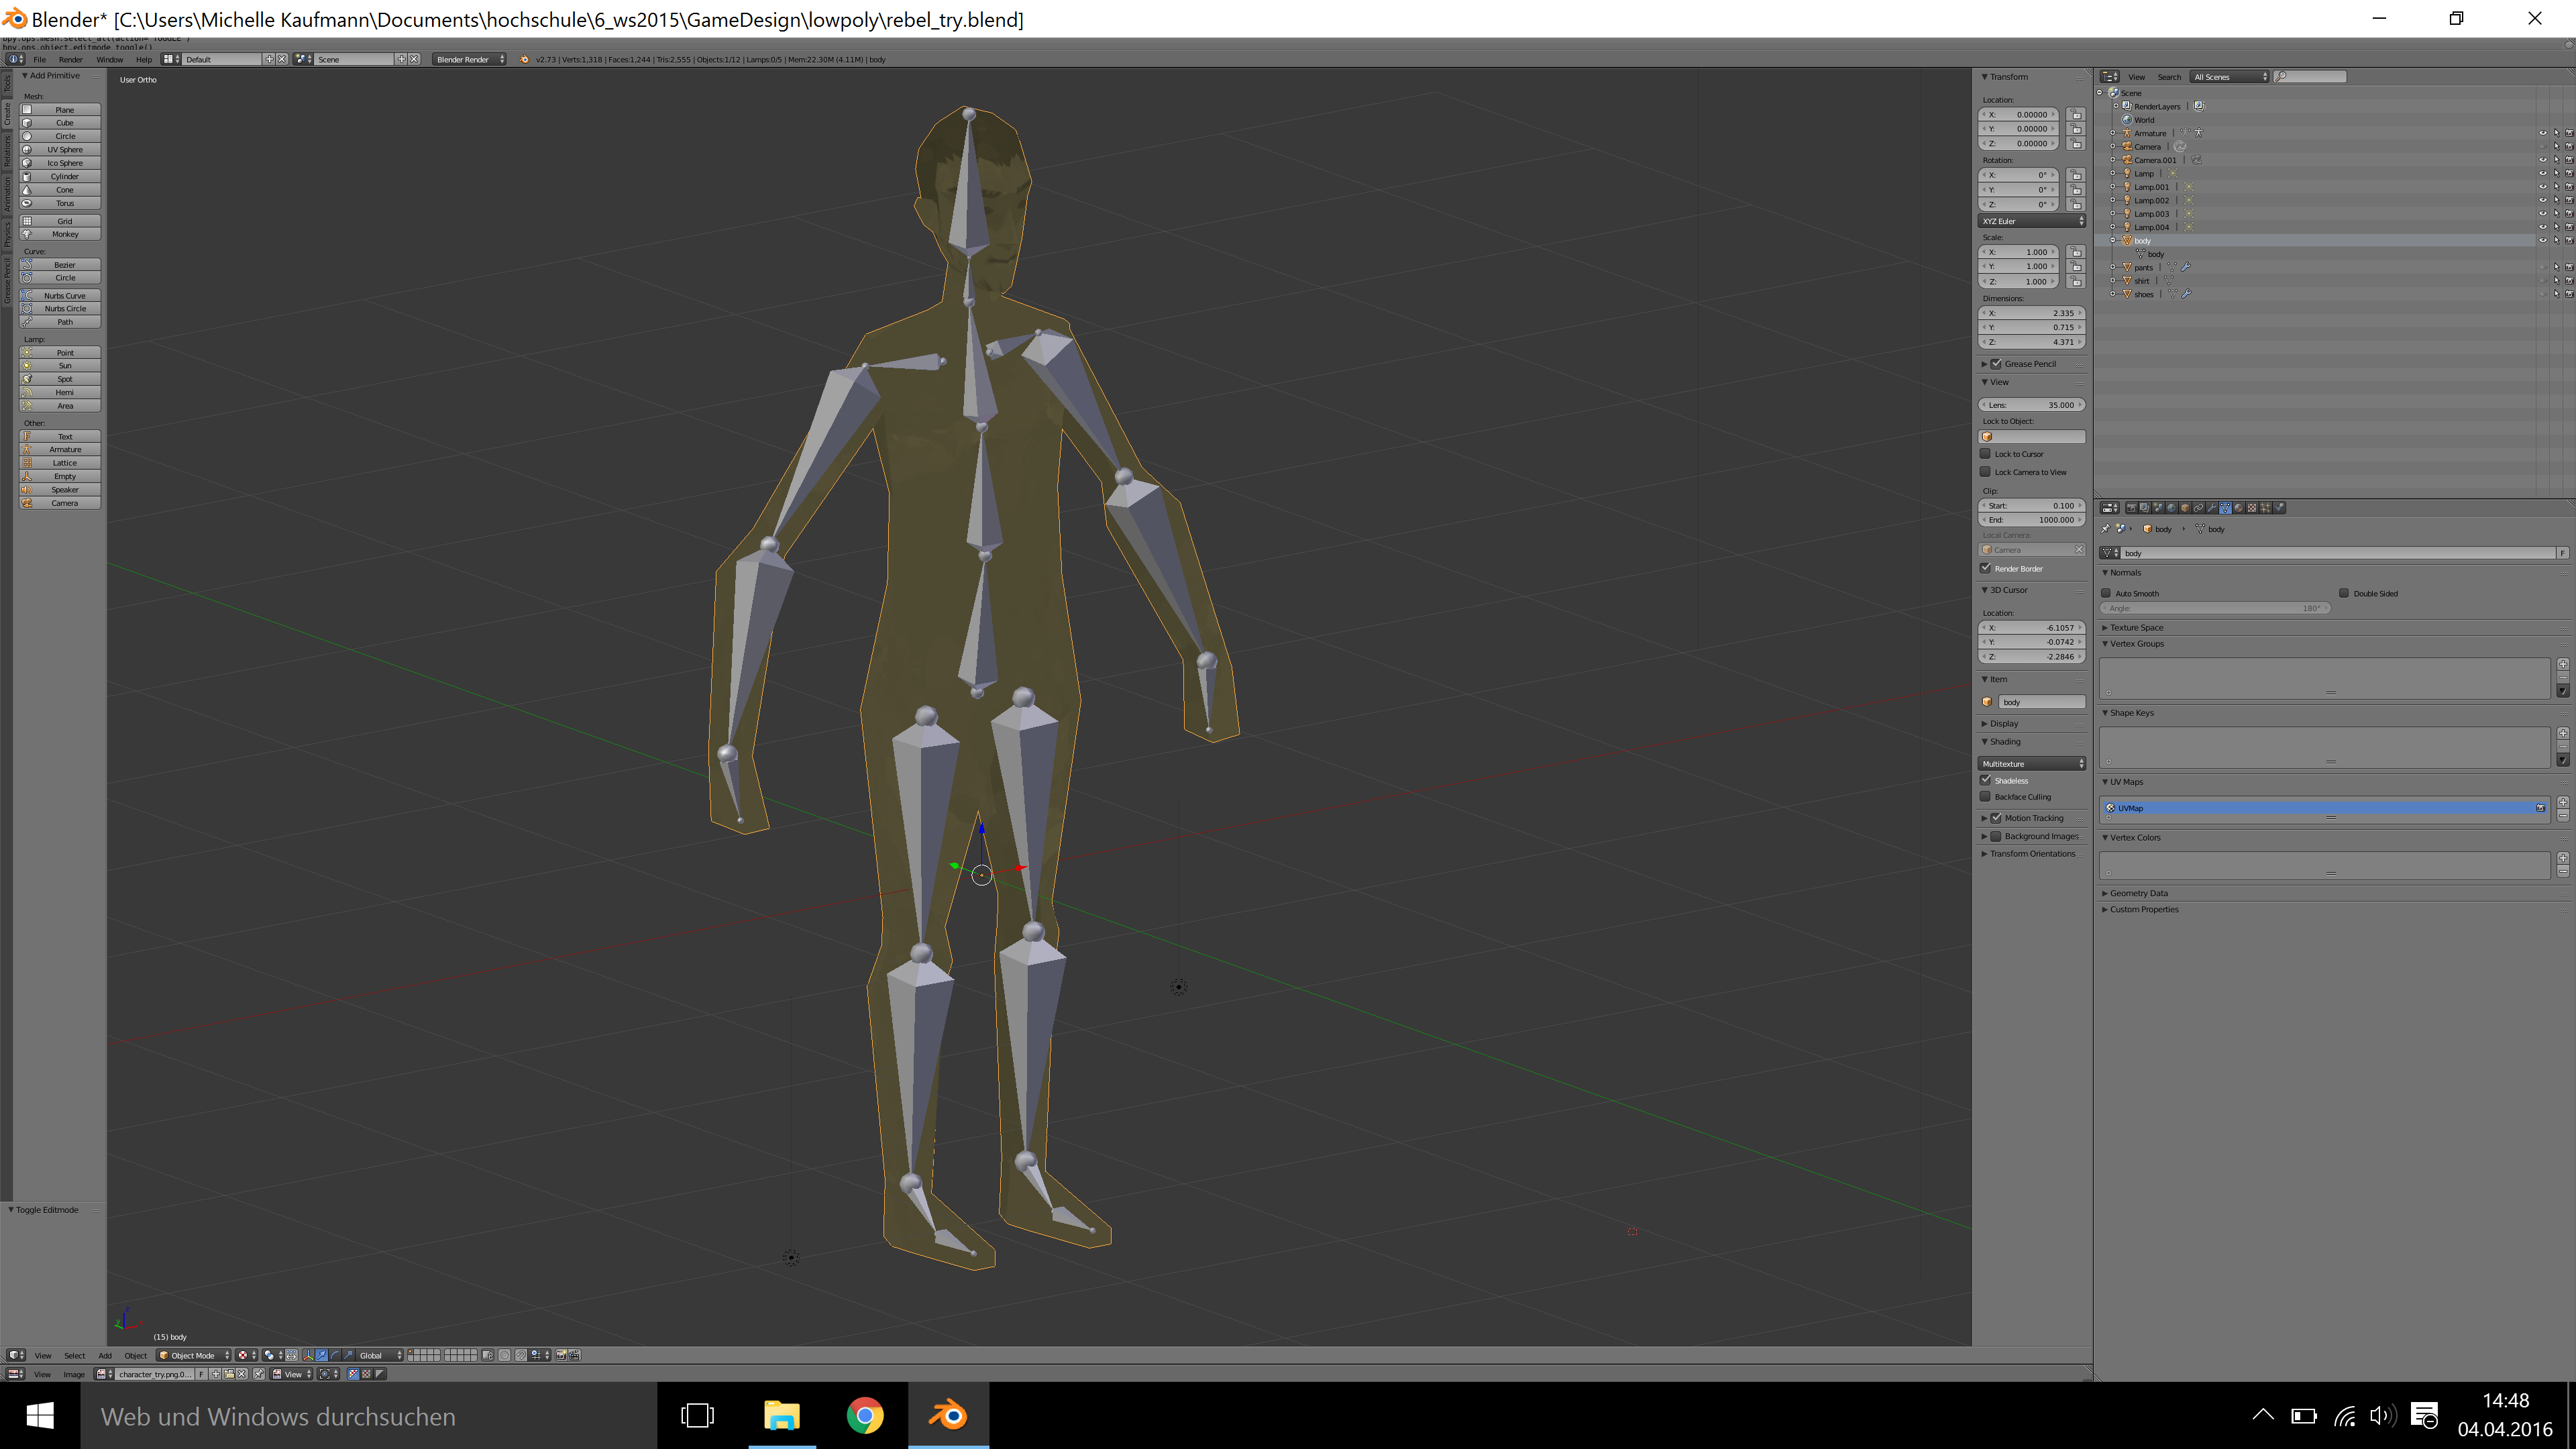
\includegraphics[height=6cm]{images/screenshot3.png}
	\caption{Charaktermodell in Blender}
	\label{fig:charmodell}
\end{figure}

\begin{figure}
	\centering
	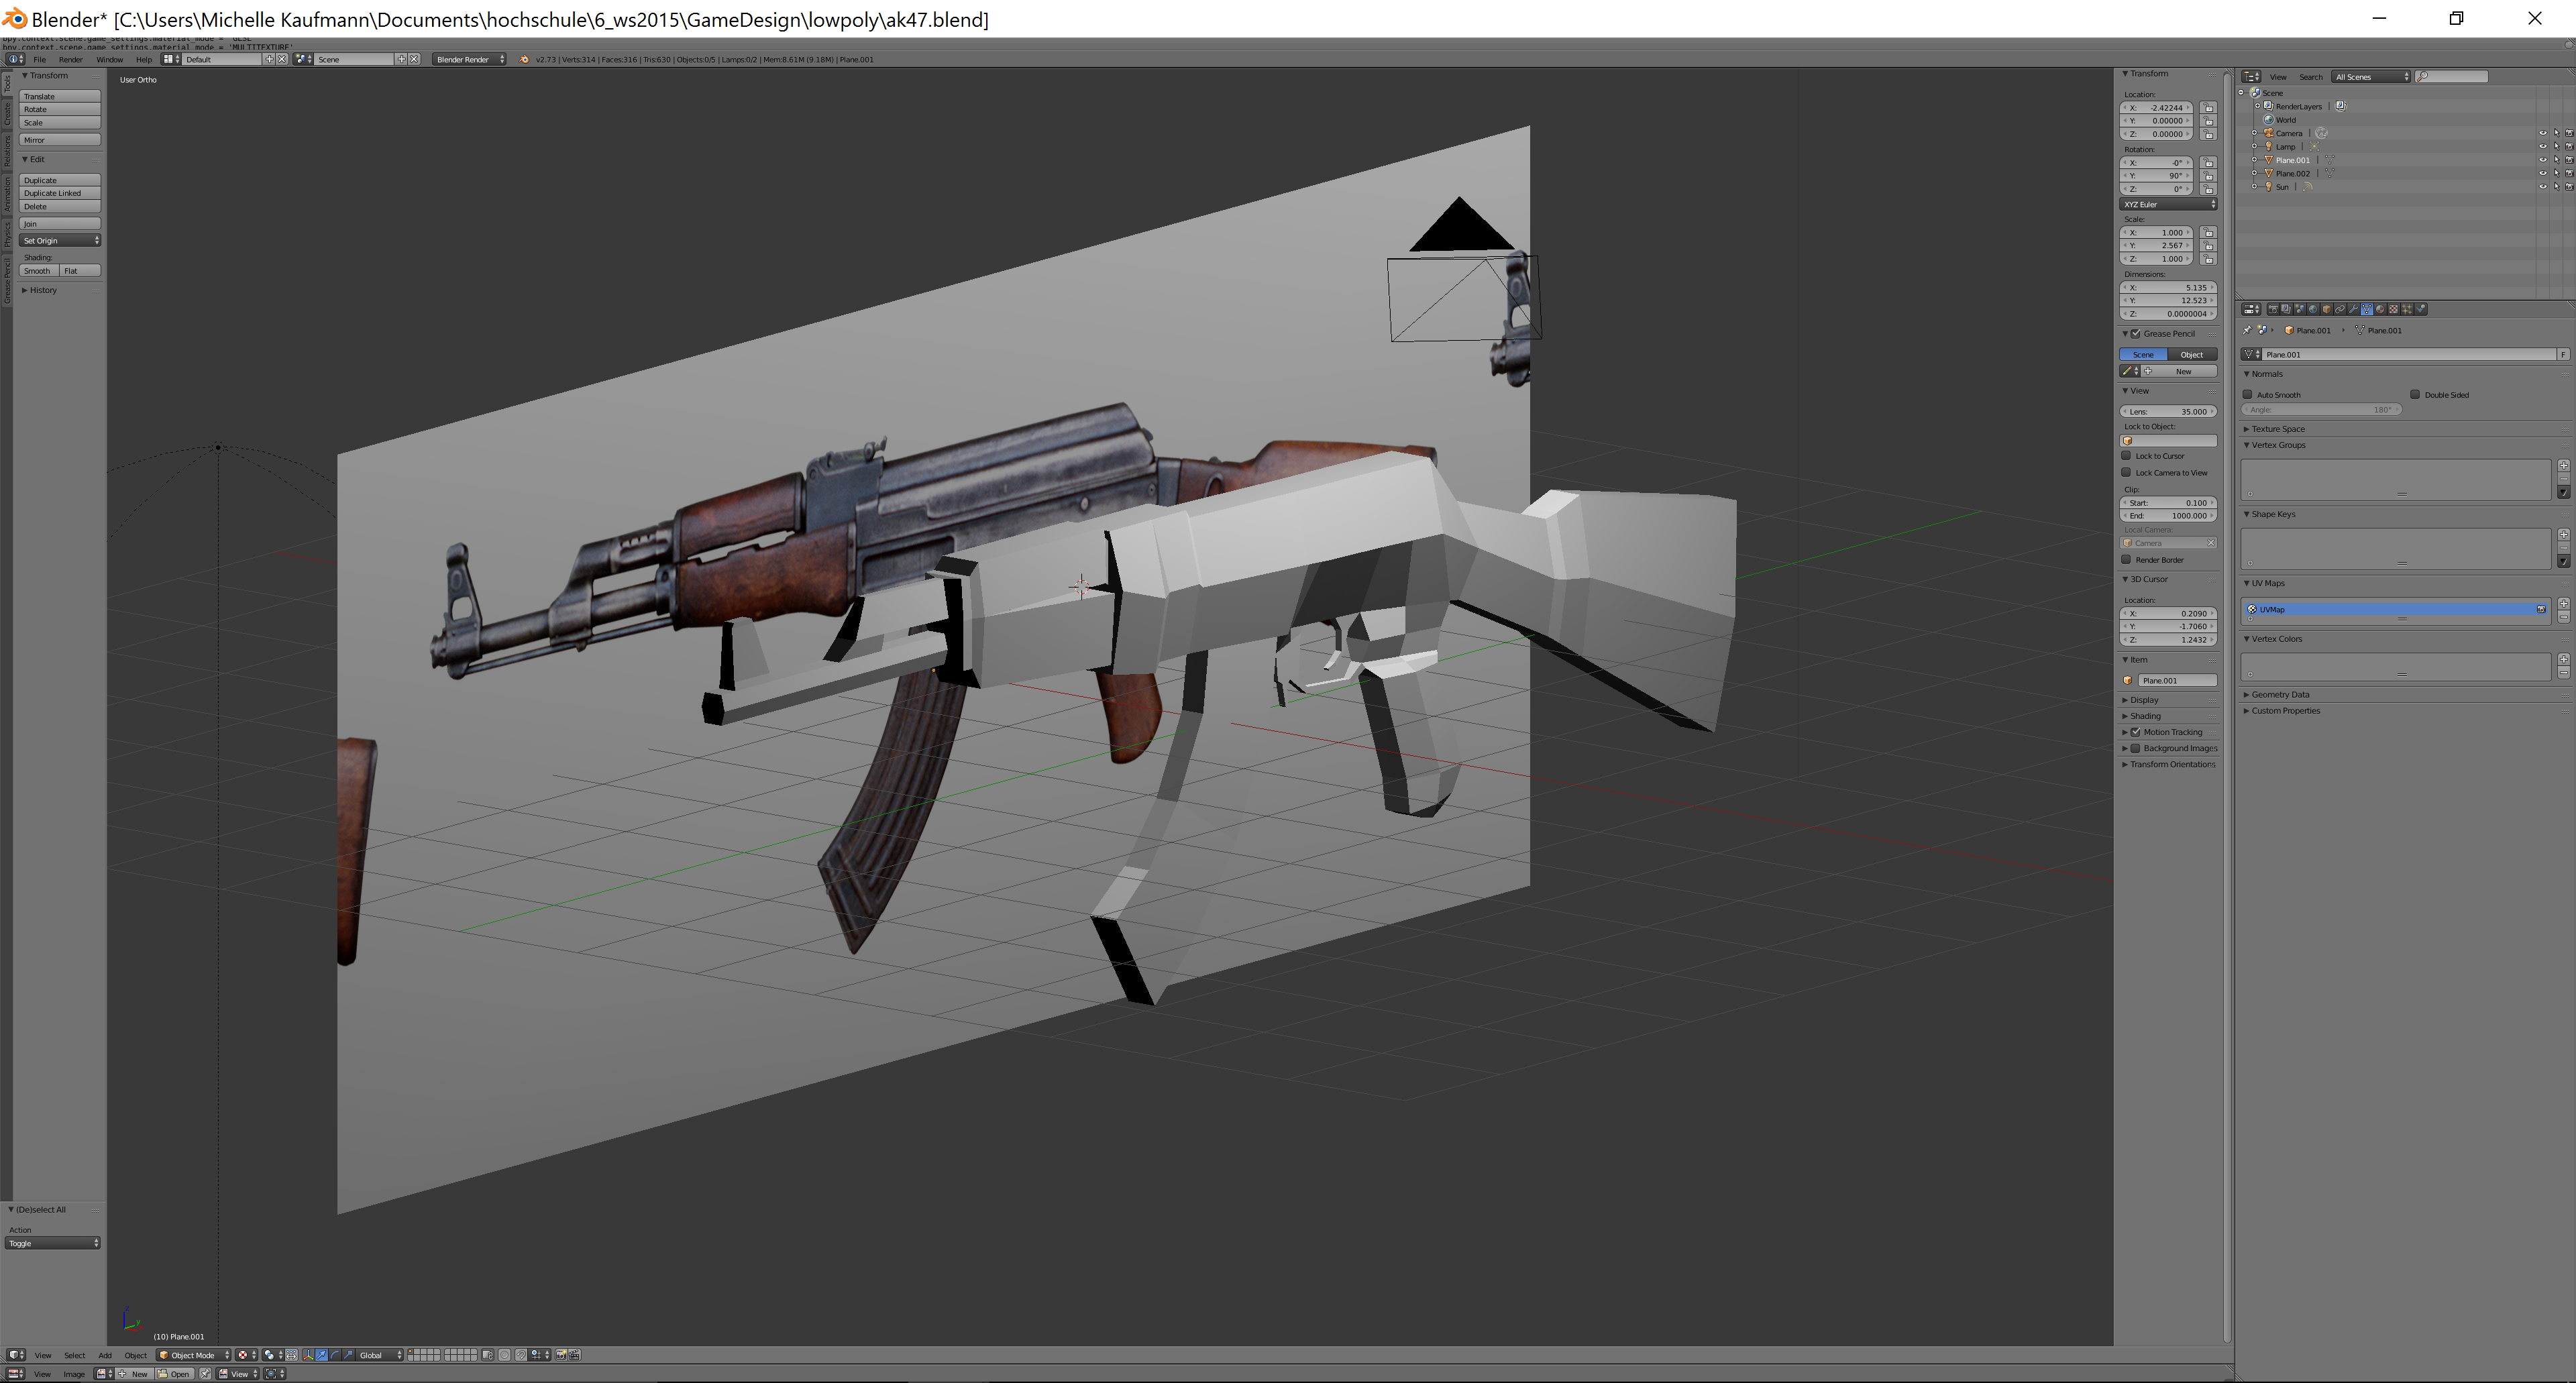
\includegraphics[height=6cm]{images/screenshot2.png}
	\caption{Waffenmodellierung in Blender}
	\label{fig:akmodel}
\end{figure}

\begin{figure}
	\centering
	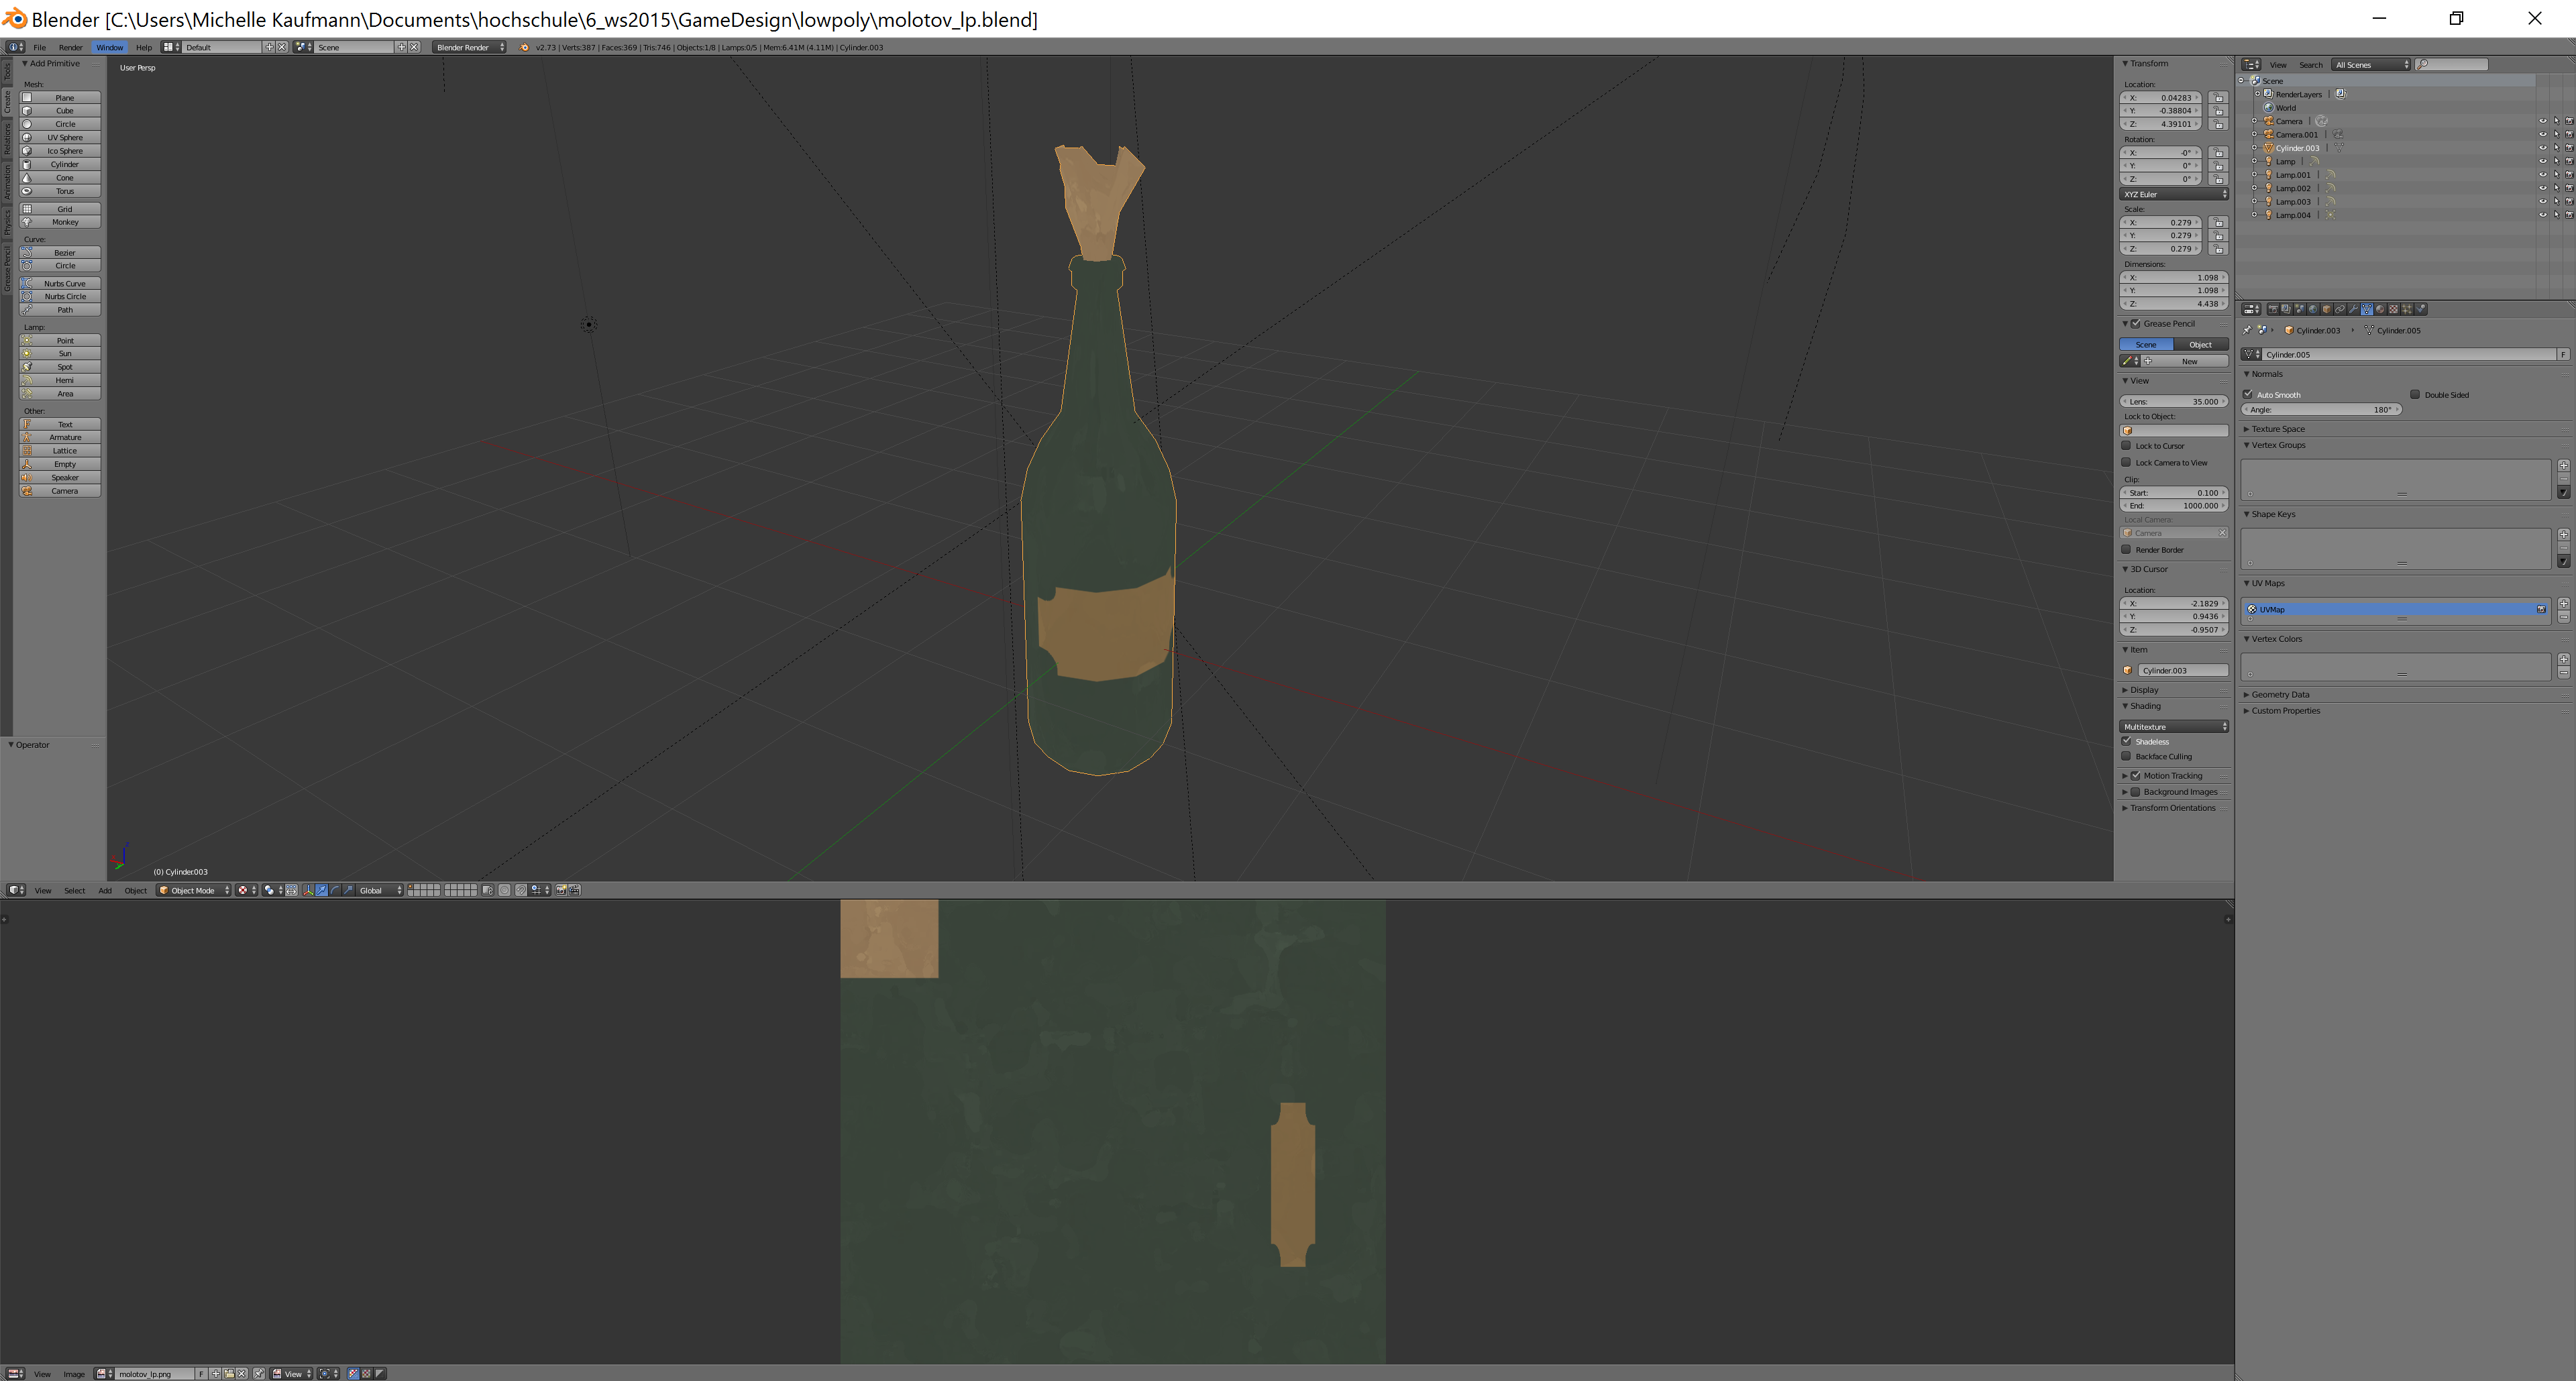
\includegraphics[height=6cm]{images/screenshot4.png}
	\caption{Propmodellierung in Blender}
	\label{fig:molotovmodel}
\end{figure}

\begin{figure}
	\centering
	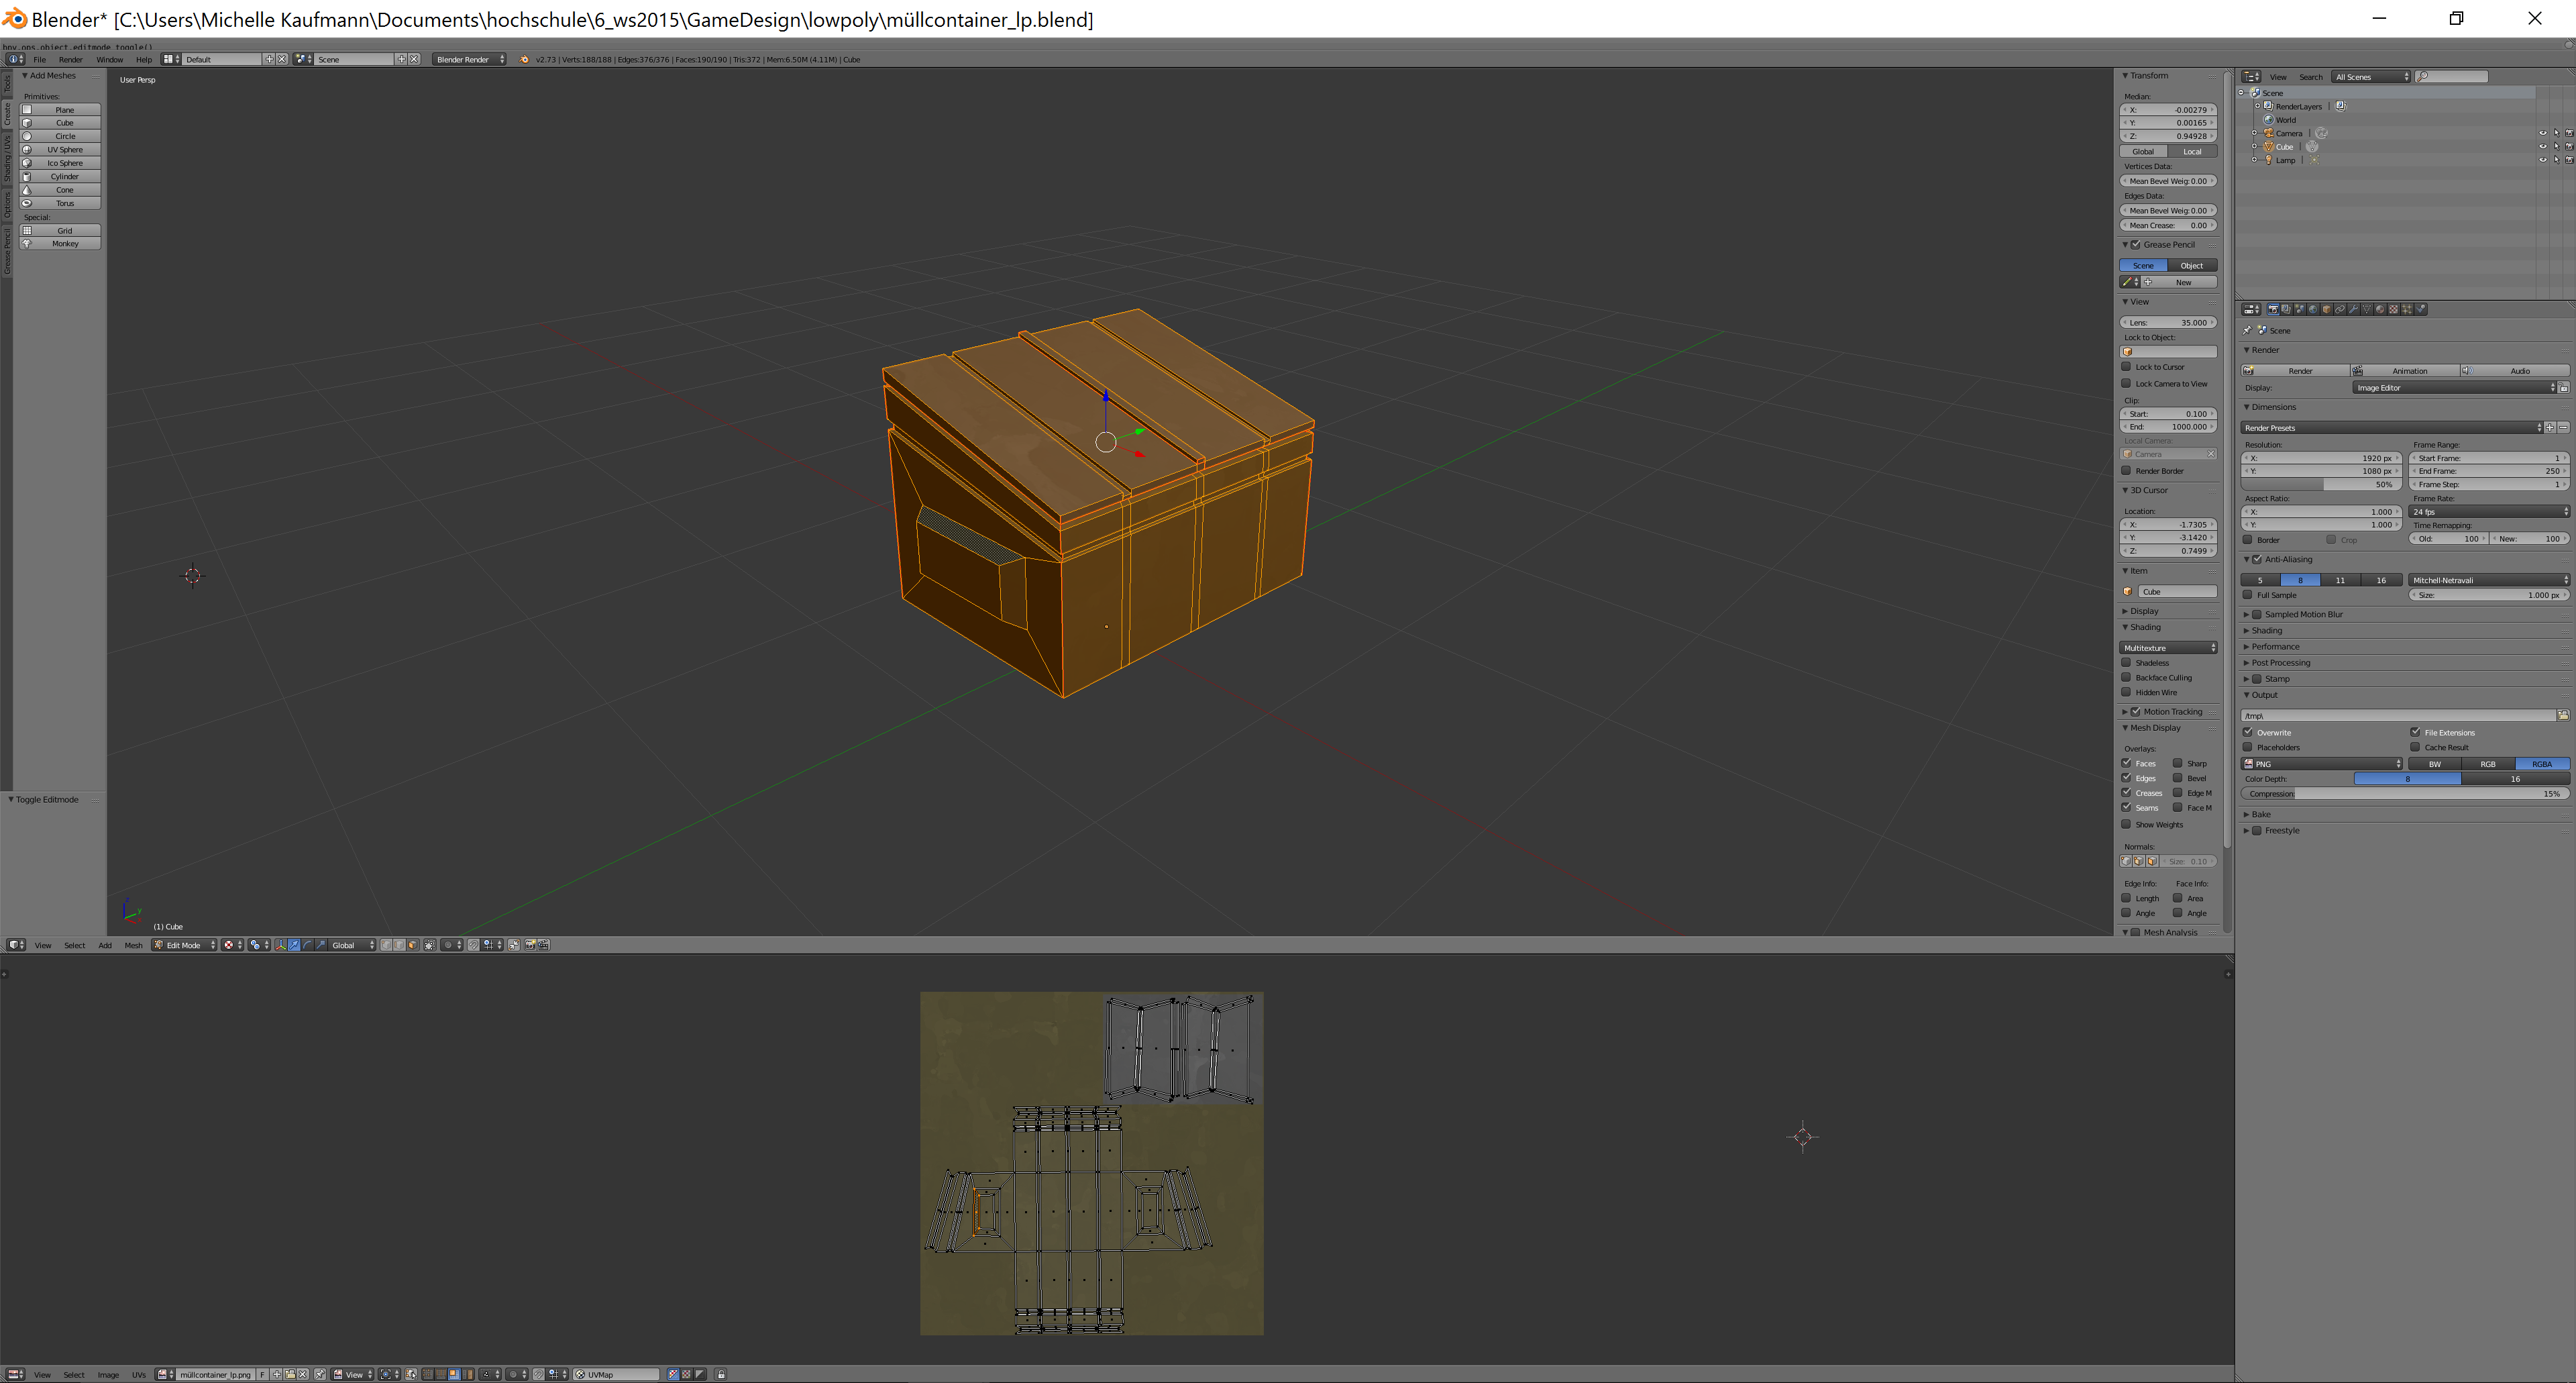
\includegraphics[height=6cm]{images/screenshot1.png}
	\caption{Propmodellierung in Blender}
	\label{fig:containermodel}
\end{figure}